\documentclass[a4paper,12pt]{article}
\usepackage{pdfpages}
\usepackage[utf8]{inputenc}
\usepackage{lipsum}
\usepackage{listings}
\usepackage{pdflscape}
\usepackage{graphicx}
\usepackage[margin=1.5cm]{geometry} % Verkleinert die R�nder
\definecolor{okgreen}{rgb}{0.0, 0.5, 0.0}

\lstdefinestyle{cppstyle}{
  language=C++,
  basicstyle=\ttfamily\tiny,
  keywordstyle=\color{blue},
  commentstyle=\textcolor{okgreen},
  stringstyle=\color{red},
  numbers=left,
  numberstyle=\tiny\color{gray},
  stepnumber=1,
  breaklines=true,
  frame=single
}

\definecolor{failred}{rgb}{0.7, 0.0, 0.0}

\lstdefinelanguage{TestOutput}{
    morekeywords={},
    morecomment=[l]{//},
    morestring=[b]",
    sensitive=false,
}

\lstdefinestyle{teststyle}{
    language=TestOutput,
    basicstyle=\ttfamily\small,
    keywordstyle=\color{black},
    commentstyle=\color{gray},
    stringstyle=\color{black},
    showstringspaces=false,
    breaklines=true,
    frame=single,
    numbers=left,
    numberstyle=\tiny\color{gray},
    postbreak=\mbox{\textcolor{red}{$\hookrightarrow$}\space},
    literate={OK}{{\textcolor{okgreen}{OK}}}2
             {Fail}{{\textcolor{failred}{Fail}}}4,
}

\begin{document}
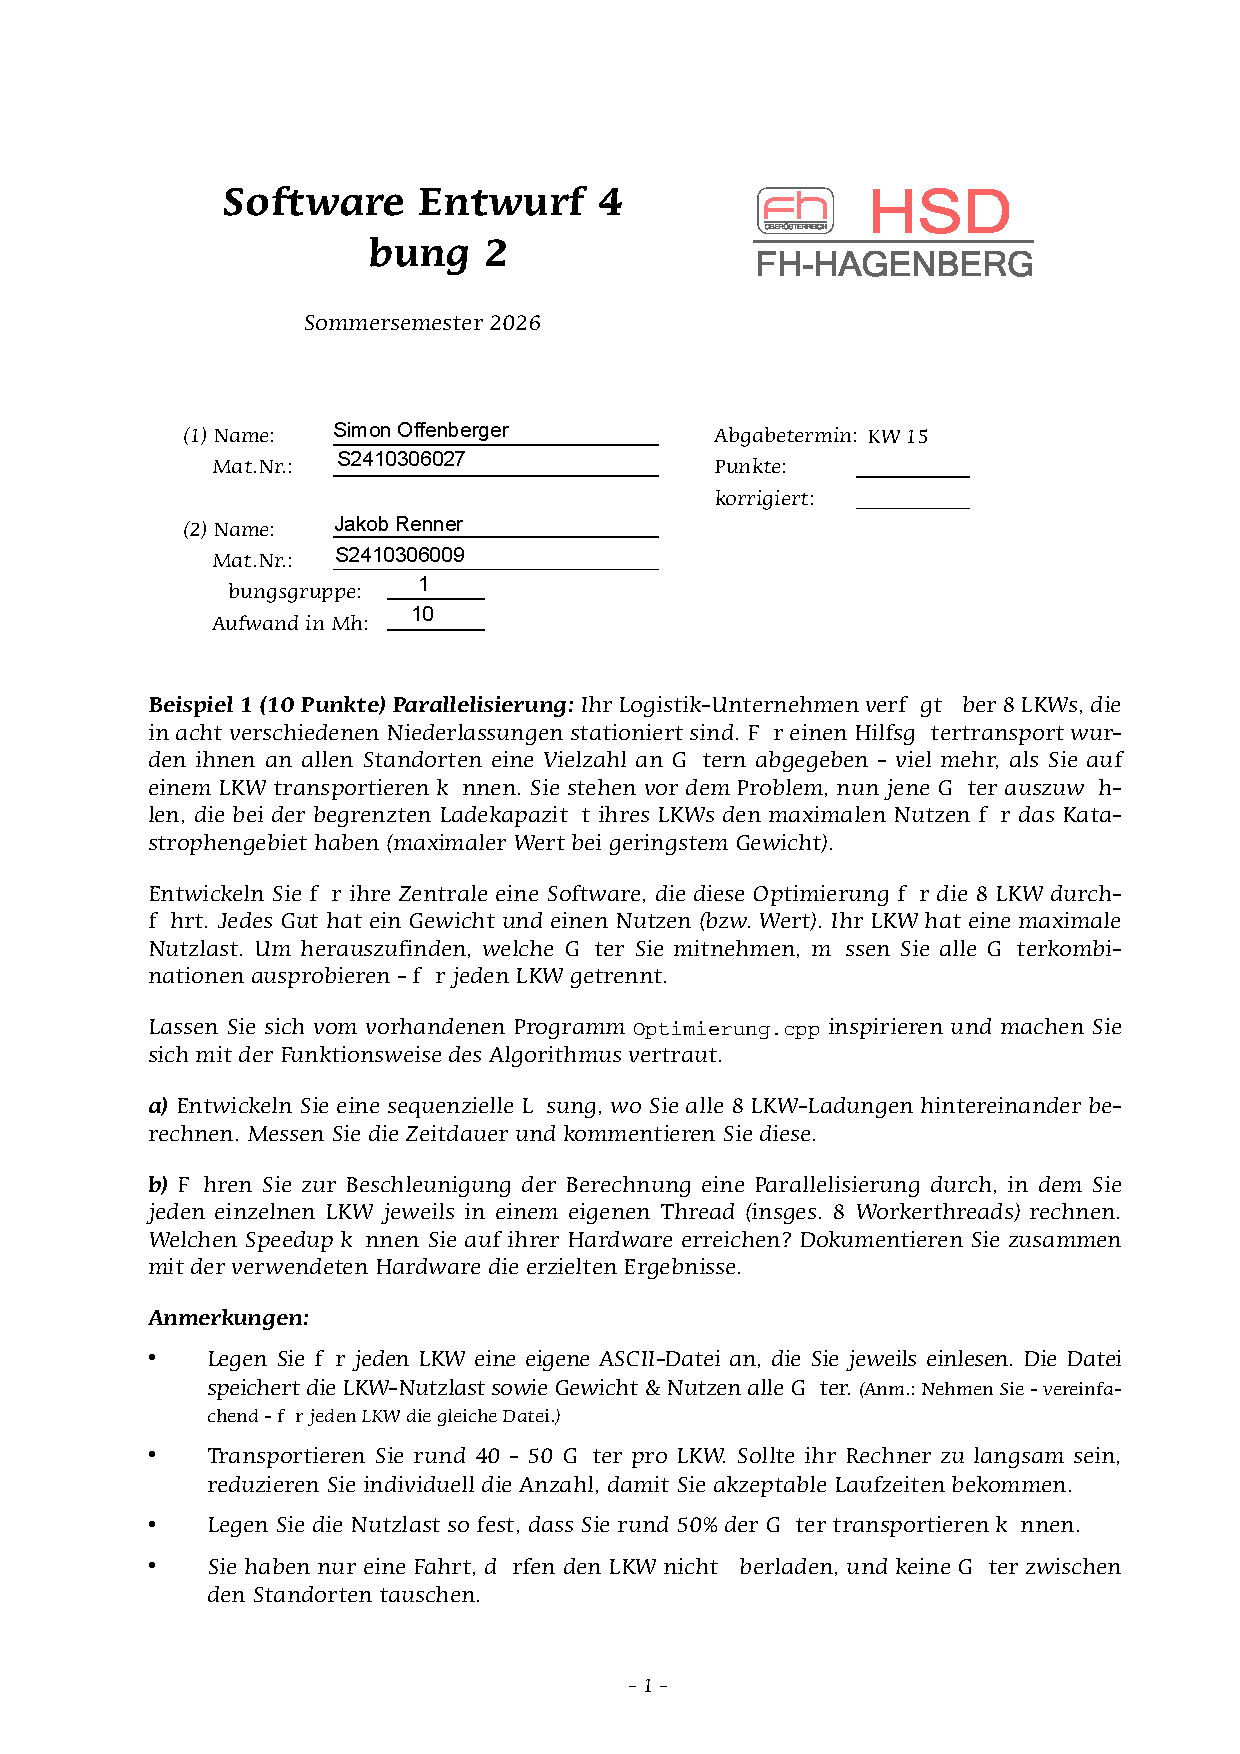
\includepdf[pages=1-3] {Uebung02_Deckblatt.pdf}
\newpage
\section{Beispiel 1 LKW:}

\section{Beispiel 2 Admin Tool:}

\subsection{Funktionsbeschreibung:}
Das Admin Tool bietet folgende Funktionen:
\begin{itemize}
		\item \textbf{OpenApp:} Öffnet eine Anwendung basierend auf dem übergebenen Pfad.
		\item \textbf{ListApps:} Listet alle laufenden Anwendungen auf.
		\item \textbf{TerminateApp:} Beendet eine Anwendung basierend auf der übergebenen PID.
		\item \textbf{ListSystemInfo:} Zeigt Informationen über das System an.
\end{itemize}

Die Funktionen sind mittels Erzeugen eines Command-Objekts ausführbar.

Im Testtreiber wurde ein einfaches Menü erstellt, welches in ähnlicher weise wie ein Konsolenmenü funktioniert.

Mit folgenden Eingaben können die Funktionen getestet werden:
\begin{itemize}
	\item \textbf{OpenApp:} "exec \textless Pfad zur Anwendung \textgreater"
	\item \textbf{ListApps:} "lsa"
	\item \textbf{TerminateApp:} "term \textless PID \textgreater"
	\item \textbf{ListSystemInfo:} "lss"
	\item \textbf{Beenden:} "exit"
\end{itemize}

Die Anwendung wird nur korrekt beendet, wenn "exit" eingegeben wird. 
Ansonsten treten Memory Leaks auf, da die Command-Objekte nicht korrekt gelöscht werden.

\subsection{Design:}
Für diese Aufgabenstellung wurde das Command Pattern angewandt.
Dazu wird ein Interface Command als Abstraktion für die verschiedenen Kommandos erstellt.
Die konkreten Kommandos (OpenApp, ListApps, TerminateApp, ListSystemInfo) implementieren dieses Interface und enthalten die jeweilige Logik für die Ausführung der Kommandos.
Die Menu-Klasse dient als Invoker, der die Kommandos verwaltet und ausführt.\\

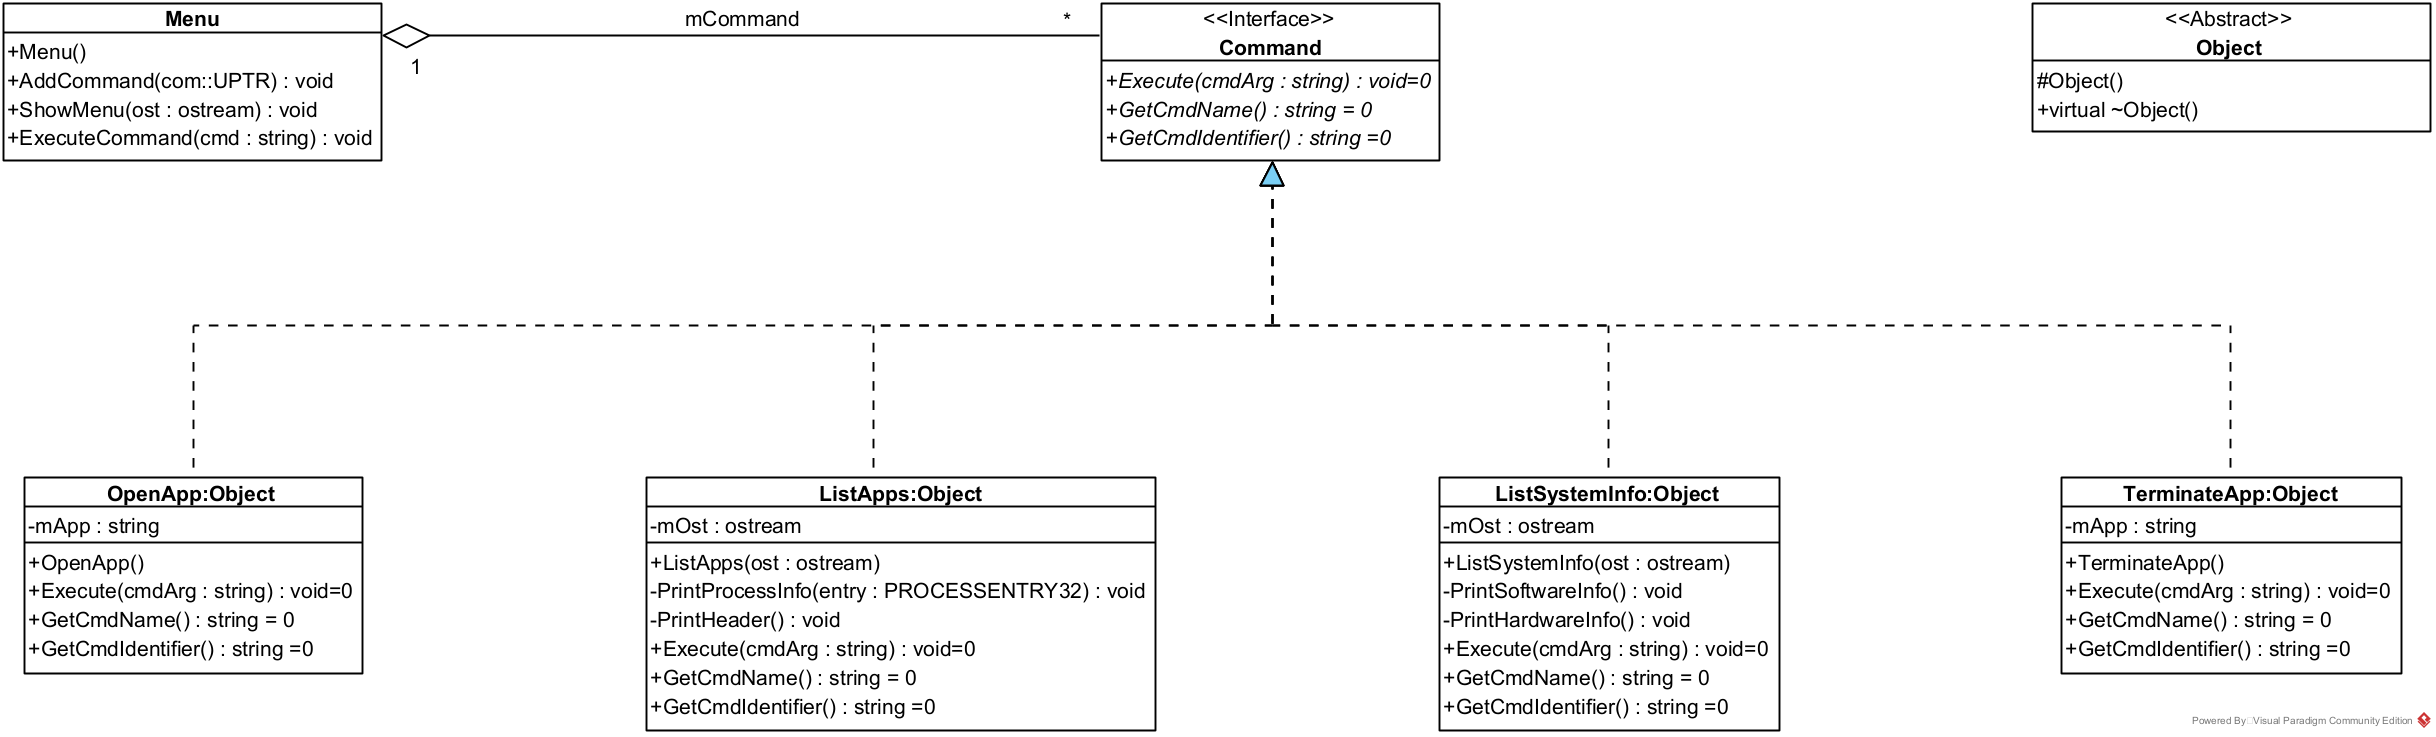
\includegraphics[width=0.8\textwidth]{./UML_AdminTool/Klassendiagramm.png}
\newpage
\subsubsection{Object.h}
\lstinputlisting[style=cppstyle]{./../AdminTool/Object.hpp}
\newpage

\subsubsection{Command.h}
\lstinputlisting[style=cppstyle]{./../AdminTool/Command.hpp}
\newpage

\subsubsection{OpenApp.h}
\lstinputlisting[style=cppstyle]{./../AdminTool/OpenApp.hpp}
\newpage

\subsubsection{OpenApp.cpp}
\lstinputlisting[style=cppstyle]{./../AdminTool/OpenApp.cpp}
\newpage

\subsubsection{ListApps.hpp}
\lstinputlisting[style=cppstyle]{./../AdminTool/ListApps.hpp}
\newpage

\subsubsection{ListApps.cpp}
\lstinputlisting[style=cppstyle]{./../AdminTool/ListApps.cpp}
\newpage

\subsubsection{TerminateApp.hpp}
\lstinputlisting[style=cppstyle]{./../AdminTool/TerminateApp.hpp}
\newpage

\subsubsection{ListSystemInfo.cpp}
\lstinputlisting[style=cppstyle]{./../AdminTool/ListSystemInfo.cpp}
\newpage

\subsubsection{ListSystemInfo.hpp}
\lstinputlisting[style=cppstyle]{./../AdminTool/ListSystemInfo.hpp}
\newpage

\subsubsection{TerminateApp.cpp}
\lstinputlisting[style=cppstyle]{./../AdminTool/TerminateApp.cpp}
\newpage

\subsubsection{Menu.hpp}
\lstinputlisting[style=cppstyle]{./../AdminTool/Menu.hpp}
\newpage

\subsubsection{Menu.cpp}
\lstinputlisting[style=cppstyle]{./../AdminTool/Menu.cpp}
\newpage

\subsubsection{OpenApp.cpp}
\lstinputlisting[style=cppstyle]{./../AdminTool/OpenApp.cpp}
\newpage

\subsubsection{Testausgabe:}
\lstinputlisting[style=teststyle]{./../AdminTool/Testoutput.txt}
\newpage
\subsubsection{Testtreiber:}
\lstinputlisting[style=cppstyle]{./../AdminTool/main.cpp}
\end{document}